\section{Requirements}
\label{sec:Requirements}

The system consists of two key components: a migration tool and a migration guide specification. This section provides an overview of the requirements and constraints for both of them. The system must meet all of them in order to be accepted. The requirements are split into functional and nonfunctional requirements. Bruegge et. al define functional requirements "[as] the interactions between the system and its environment independent of its implementation" \cite{bruegge_object-oriented_2010}. The authors thereby describe users and external systems as part of a system's environment. Furthermore, Bruegge et al. define nonfunctional requirements "as aspects of the system that are not directly related to the functional behavior of the system" \cite{bruegge_object-oriented_2010}. They further divide nonfunctional requirements into quality requirements and constraints. 

\subsection{Functional Requirements}
\label{subsec:FunctionalRequirements}
 
 In order to enable the implementation of the workflow shown in Figure \ref{fig:newWorkflow}, both, the functional requirements of the Web API consumers and providers must be taken into account. 

\begin{itemize}[itemindent=-4pt, leftmargin=34pt, align=left]
    \item [FR1\hphantom{1}] \customlabel{fr:MigGuide}{Developing a specification for a machine-readable migration guide (FR1)} \textbf{Development of a specification for a machine-readable migration guide:} The machine-readable migration guide needs to contain all necessary information regarding changes made to the Web API. Additionally, it must provide fields to specify important meta-data like versioning information. The format of the migration guide must allow the specification of simple and complex data structures. They are required to model hierarchies within the guide or hierarchical types provided by a Web API. Changes stated within the migration guide must be distinguishable from one another by their structure. Depending on its type, a change must include fields that contain information on how to adapt the client code to maintain compatibility with the Web API.
    \item [FR2\hphantom{1}] \customlabel{fr:Configuration}{Configuration} \textbf{Provide configuration option:} A user can configure the system by providing command-line parameters or a configuration file. If applicable, a default value is used in case of a missing configuration. For each API and project, an individual configuration can be applied.
    \item [FR3\hphantom{1}] \customlabel{fr:GenLib}{Generate a client library from service specification} \textbf{Generating a client library from service specification:} A user provides a Web API specification URI as input to generate a client library which can be used by the client application. The input can either be issued locally as a file or can be remotely retrieved from the web service.
    \item [FR4\hphantom{1}] \customlabel{fr:Facade}{Providing a facade to maintain API consistency (FR4)} \textbf{Provide a facade to maintain API consistency:} A user accesses the library's functionality via a generated facade to ensure a consistent view of the API. It mimics the original interface as it uses the same method signatures and exposes them to the client application.
     \item [FR5\hphantom{1}] \customlabel{fr:AdaptFacade}{Self-adapting facade for API evolution (FR5)}
     \textbf{Self-adapting facade for API evolution:} The system automatically resolves the current version of the web service and its corresponding migration guide. If the retrieved API version differs from the local API version, the system adapts the facade according to the migration guide. As a result, users automatically receive API-related changes in their application code.
     \item [FR6\hphantom{1}] \customlabel{fr:CIInteg}{Integrate system in CI/CD}
     \textbf{Integrate system in CI/CD:} The tool will be integrated into the CI pipeline of the client application to ensure the highest level of automation. Alternatively it can be used locally via its \textit{\ac{CLI}}.
     \item [FR7\hphantom{1}] \customlabel{fr:GitInteg}{Integrate output via Git}
     \textbf{Integrate output via Git:} The modified library will be published via git pull request into the client application's repository. By publishing it, the library's version number will be incremented according to semantic versioning principles.
     \item [FR8\hphantom{1}] \customlabel{fr:MigStrategy}{Specify migration strategy}
     \textbf{Specify migration strategy:} A user can specify the migration strategy for non-migratable changes such as deletion of functionality without replacement. The selected strategy can be either provided via command-line parameters or using the configuration file. 
          \item [FR9\hphantom{1}] \customlabel{fr:OutputLang}{Specify output language}
     \textbf{Specify output language:} A user can specify the programming language in which the target library is generated. The selected output language can be either provided via command-line parameters or using the configuration file. 
\end{itemize}

\subsection{Artifacts}
\label{subsec:Artifacts}

To illustrate the artifacts from FR1 and FR4, Figure \ref{fig:migGuide} shows our proposed structure for a machine-readable migration guide and Figure \ref{fig:outcome} demonstrates the architectural composition of the code generated by our system.

\begin{figure}[h]
	\centering{
		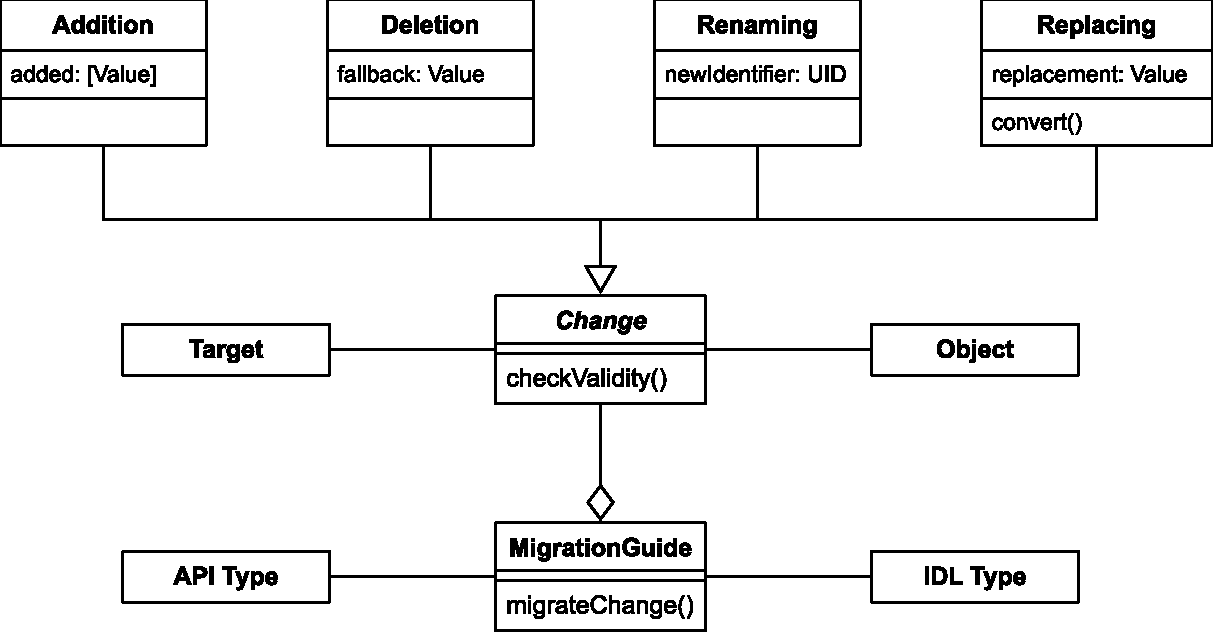
\includegraphics[width=135mm]{images/cd_migration_guide.pdf}
		\caption{Proposed structure of a machine-readable migration guide}
		\label{fig:migGuide}
	}
\end{figure}

A migration guide is responsible for migrating different types of changes that might occur due to Web API evolution. Each change must contain an identification of the object which is changed and the specific target of the change. For example, if a method parameter was changed, the method is the change object and the parameter is the change target.

\begin{figure}[!h]
	\centering{
		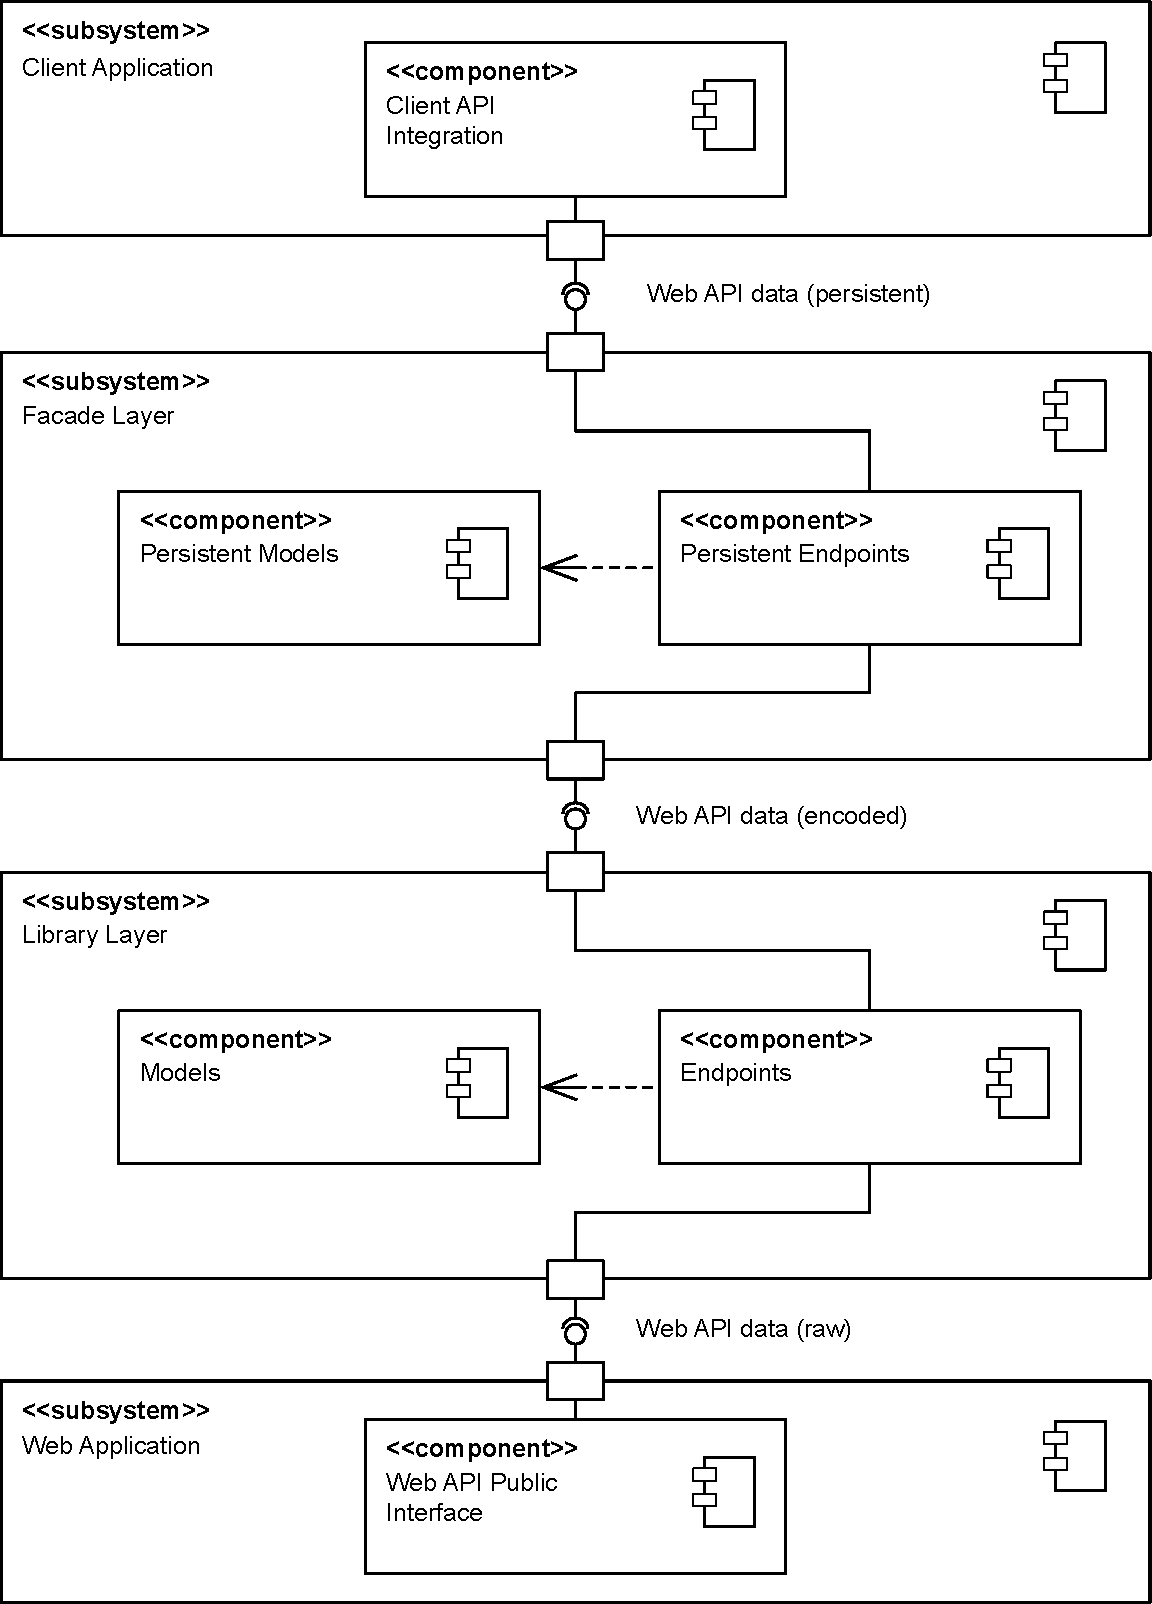
\includegraphics[width=130mm]{images/output_subsystem.pdf}
		\caption{Proposed architecture of change-proof Web API integration}
		\label{fig:outcome}
	}
\end{figure}

The output of our system is designed in a layered architectural style in order to incorporate changes made to the Web API without affecting the client application. Due to the fact that Web APIs are already integrated using a layered network architecture, introducing additional layers does not affect current development practices. The library subsystem is a local representation of the Web API and provides its services only to the facade subsystem. The facade subsystem uses them to issue HTTP requests to the Web API while maintaining a stable interface to the client application. When changes are introduced to the Web API, the library subsystem gets updated accordingly and the API contract between the library and facade subsystems is broken. For fixing the API contract, all changes stated in the migration guide modify the internal functionality of the facade subsystem without altering any publicly exposed interfaces. 

\subsection{Nonfunctional Requirements}
\label{subsec:NonfunctionalRequirements}
The following requirements were defined to ensure a high quality system. As described in \cite{bruegge_object-oriented_2010}, each requirement relates to one or more of the categories usability, reliability or supportability. According to the authors, supportability includes adaptability and maintainability.

\begin{itemize}[itemindent=-13pt, leftmargin=43pt, align=left]
    \item [NFR1\hphantom{1}] \customlabel{nfr:CodeStyle}{NFR1 (Code Style)} \textbf{Code Style:} All code generated by the system must follow a linting ruleset predefined in a configuration file to increase maintainability.
    \item [NFR2\hphantom{1}] \customlabel{nfr:ClientDocumentation}{NFR2} \textbf{Documentation of facade:} To increase usability for client application developers, the facade's public interface will be documented using code comments. These comments explain the usage of the Web API and are derived from its IDL document.
    \item [NFR3\hphantom{1}] \customlabel{nfr:SystemDocumentation}{NFR3} \textbf{Documentation of system:} To increase maintainability, the system will be documented using code comments. Documentation will be auto-gen\-erated and summarized in the \texttt{README.md} file.
    \item [NFR4\hphantom{1}] \customlabel{nfr:TestCoverage}{Test Coverage (NFR4)} \textbf{Test coverage:} To ensure the system's robustness, unit tests must be provided for all supported migration types. Additionally, unit test must be provided with respect to different migration strategies. Special attention needs to be paid to edge cases.
    \item [NFR5\hphantom{1}] \customlabel{nfr:Coloring}{NFR5}
    \textbf{Coloring of key messages:} Key output messages of the system will be highlighted using coloring schemes to increase usability.
    \item [NFR6\hphantom{1}] \customlabel{nfr:Help}{NFR6}
    \textbf{Help messages:} The system provides detailed instructions on how to use its command-line interface. The help will be available via \texttt{help} command. This ensures that users are able to easily learn how to operate the system.
    \item [NFR7\hphantom{1}] \customlabel{nfr:CodeVersion}{NFR7}
    \textbf{Code version:} The system is constrained to issuing language-specific library code in the language's current major version. This improves adaptability when client applications are using the latest version of a programming language.
    \item [NFR8\hphantom{1}] \customlabel{nfr:Dependencies}{NFR8}
    \textbf{Dependency Management:} Language-specific implementations are required to use a dependency manager to manage all third party libraries. Using a dependency manager increases maintainability significantly because dependency meta information provides a single source of truth.
        \item [NFR9\hphantom{1}] \customlabel{nfr:MigGuideFormat}{NFR9 (Migration Guide Format)}
    \textbf{Migration guide format:} The migration guide needs to be specified in a human-readable format which web developers are familiar with. Using a domain-specific language increases acceptance and usability especially for debugging and manual inspection. Additionally, utilizing a format that is already widely used in the software development industry has the advantage that IDEs provide convenient features such as syntax highlighting or auto-completion.
        \item [NFR10\hphantom{1}] \customlabel{nfr:UserInput}{NFR10}
    \textbf{Handling user input:} Missing or incorrect configuration parameters trigger a detailed error message so that the user can easily examine and correct the configuration.
\end{itemize}

\subsection{Constraints}
\label{subsec:Constraints}

For the system to work properly, some constraints have to be fulfilled. A constraint is a nonfunctional requirement that has been specified in advance by external factors and must be reconciled with other affected design decisions \cite{bass_software_2013}.

\begin{itemize}[itemindent=-13pt, leftmargin=43pt, align=left]
    \item [C1\hphantom{1}] \customlabel{nfr:Legal}{C1} \textbf{Legal requirements}: All dependencies must be available under MIT license regulations so that the system can also be published under the MIT license.
    \item [C2\hphantom{1}] \customlabel{nfr:Operations}{NFR2} \textbf{Operations requirements}: An IDL document describing the public interface of an API must be available in order to generate library code. Furthermore, both the API consumers and producers need to follow semantic versioning\footnote{see https://semver.org/} principles.
    \item [C3\hphantom{1}] \customlabel{nfr:Implementation}{NFR3} \textbf{Implementation requirements}: API consumers have to use GitHub as their version control system to use the system as a GitHub action in their CI/CD pipeline. Additionally, it is provided as a command-line program without a graphical user interface. This enables local execution or integration into other CI/CD tools.
\end{itemize}
